%\documentclass[handout]{beamer}
\documentclass{beamer}

\mode<presentation>
{
\usetheme{default}
\usefonttheme[onlymath]{serif}
%\usetheme{Singapore}
%\usetheme{Warsaw}
%\usetheme{Malmoe}
% \useinnertheme{circles}
% \useoutertheme{infolines}
% \useinnertheme{rounded}

\setbeamercovered{transparent=5}
}

\usepackage[english]{babel}
\usepackage[latin1]{inputenc}
\usepackage{bm,textpos,alltt,listings,multirow,ulem,siunitx}

% font definitions, try \usepackage{ae} instead of the following
% three lines if you don't like this look
\usepackage{mathptmx}
\usepackage[scaled=.90]{helvet}
%\usepackage{courier}
\usepackage[T1]{fontenc}
\usepackage{tikz}
\usetikzlibrary[shapes.arrows,arrows,shapes.misc]

% \usepackage{pgfpages}
% \pgfpagesuselayout{4 on 1}[a4paper,landscape,border shrink=5mm]

\usepackage{slashbox,multirow,listings,booktabs}
\usepackage{xspace}
\makeatletter
\DeclareRobustCommand\onedot{\futurelet\@let@token\@onedot}
\def\@onedot{\ifx\@let@token.\else.\null\fi\xspace}
\def\eg{{e.g}\onedot} \def\Eg{{E.g}\onedot}
\def\ie{{i.e}\onedot} \def\Ie{{I.e}\onedot}
\def\cf{{c.f}\onedot} \def\Cf{{C.f}\onedot}
\def\etc{{etc}\onedot}
\def\vs{{vs}\onedot}
\def\wrt{w.r.t\onedot}
\def\dof{d.o.f\onedot}
\def\etal{{et al}\onedot}
\makeatother

\usepackage{tikz}
\usetikzlibrary[shapes,shapes.arrows,arrows,shapes.misc,fit,positioning]

\usepackage{siunitx}
\DeclareSIUnit\year{a}
\DeclareSIUnit\byte{B}
\sisetup{retain-unity-mantissa = false}

\usepackage{fancyvrb}
\usepackage{minted}
\newminted{c}{gobble=2}
\newminted{python}{gobble=2}
%\newmint[cverb]{c}{} 
\newcommand\cverb[1][]{\SaveVerb[%
    aftersave={\textnormal{\UseVerb[#1]{vsave}}}]{vsave}}
\newcommand\cfunc[1][]{\SaveVerb[%
    aftersave={\textnormal{\UseVerb[#1]{vsave}\texttt{()}}}]{vsave}}
\newcommand\pyverb[1][]{\SaveVerb[%
    aftersave={\textnormal{\UseVerb[#1]{vsave}}}]{vsave}}
\def\asm#1{{\tt #1}}
\def\code#1{{\tt #1}}
\def\shell#1{{\tt \$ #1}}

\newcommand\email[1]{{\href{mailto:#1}{\nolinkurl{#1}}}}

\newcommand{\II}{\mathcal{I}}
\newcommand{\C}{\mathbb{C}}
\newcommand{\D}{\mathcal{D}}
\newcommand{\EE}{\mathcal{E}}
\newcommand{\F}{\mathcal{F}}
\newcommand{\I}{\mathcal{I}}
\newcommand{\N}{\mathcal{N}}
\newcommand{\PP}{\mathcal{P}}
\newcommand\Ppc{\ensuremath{\mathsf P}}
\newcommand{\bigO}{\ensuremath{\mathcal{O}}}
\newcommand{\R}{\mathbb{R}}
\newcommand{\Rz}{\mathcal{R}}
\newcommand{\QQ}{\mathcal Q}
\newcommand{\VV}{\mathcal V}
\newcommand{\ASM}{\mathrm{ASM}}
\newcommand{\RASM}{\mathrm{RASM}}

\newcommand{\kb}{\tt}
\newcommand{\Pk}[1]{\ensuremath{P_{#1}}}
\newcommand{\Qk}[1]{\ensuremath{Q_{#1}}}
\newcommand{\Pkdisc}[1]{\ensuremath{P_{#1}^{\text{disc}}}}
\newcommand{\Qkdisc}[1]{\ensuremath{Q_{#1}^{\text{disc}}}}
\newcommand{\blue}{\textcolor{blue}}
\newcommand{\green}{\textcolor{green!70!black}}
\newcommand{\red}{\textcolor{red}}
\newcommand{\brown}{\textcolor{brown}}
\newcommand{\cyan}{\textcolor{cyan}}
\newcommand{\magenta}{\textcolor{magenta}}
\newcommand{\yellow}{\textcolor{yellow}}
\newcommand{\mini}{\mathop{\rm minimize}}
\newcommand{\st}{\mbox{subject to }}
\newcommand{\lap}{\Delta}
\newcommand{\grad}{\nabla}
\newcommand\mtab{\hspace{\stretch{1}}}
\newcommand\ud{\,\mathrm{d}}
\newcommand\bslash{{$\backslash$}}
\newcommand\half{{\frac 1 2}}
\newcommand{\abs}[1]{\left\lvert #1 \right\rvert}
\newcommand{\bigabs}[1]{\big\lvert #1 \big\rvert}
\newcommand{\norm}[1]{\left\lVert #1 \right\rVert}
\newcommand\oneitem[1]{\begin{itemize} \item #1 \end{itemize}}
\newcommand\pfrak{{\mathfrak p}}
\newcommand\nfrak{{\mathfrak n}}
\newcommand\ff{\bm f}
\newcommand\mm{\bm m}
\newcommand\nn{\bm n}
\newcommand\uu{\bm u}
\newcommand\vv{\bm v}
\newcommand\ww{\bm w}
\newcommand\DD{D}
\newcommand{\tcolon}{\!:\!}
\DeclareMathOperator{\sgn}{sgn}
\DeclareMathOperator{\card}{card}
\DeclareMathOperator{\trace}{tr}
\DeclareMathOperator{\erf}{erf}
\DeclareMathOperator{\sspan}{span}
\renewcommand{\bar}{\overline}
% \DeclareMathOperator{\divergence}{div}
% \renewcommand\div\divergence
\renewcommand{\div}{{\nabla \cdot}}
\newcommand\spliceop{\leftrightsquigarrow}
\newcommand\splice[5]{{#1} \overset{#5}{\underset{#3,#4}{\leftrightsquigarrow}} {#2}}
\newcommand{\ip}[2]{{\left\langle #1, #2 \right\rangle}}
\newcommand{\Linfty}{{L^\infty}}

% Dimensionless numbers
\newcommand{\Peclet}{{\mathrm{Pe}}}
\newcommand{\Reynolds}{{\mathrm{Re}}}
\newcommand{\Rayleigh}{{\mathrm{Ra}}}
\newcommand{\Mach}{{\mathrm{Ma}}}
\newcommand{\Prandtl}{{\mathrm{Pr}}}
\newcommand{\Grashof}{{\mathrm{Gr}}}

\newcommand{\PETSc}{{PETSc}}
\newcommand{\Dohp}{{Dohp}}
\newcommand\libmesh{\texttt{libMesh}}
\newcommand\dealii{\texttt{Deal.II}}
\newcommand\MatMult{\cverb|MatMult|}
\newcommand\MatSolve{\cverb|MatSolve|}
\newcommand{\secref}[1]{{Section~\ref{#1}}}
\newcommand{\chapref}[1]{{Chapter~\ref{#1}}}
\newcommand{\figref}[1]{{Figure~\ref{#1}}}
\newcommand{\tabref}[1]{{Table~\ref{#1}}}
\newcommand\AIJ{{\cverb|AIJ|}}
\newcommand\AIJInode{\cverb|AIJ|/\cverb|Inode|}
\newcommand\BAIJ[1][]{\ifthenelse{\equal{#1}{}}{\cverb|BAIJ|}{\ensuremath{\cverb|BAIJ|(#1)}}}
\newcommand\SBAIJ[1][]{\ifthenelse{\equal{#1}{}}{\cverb|SBAIJ|}{\ensuremath{\cverb|SBAIJ|(#1)}}}
\newcommand\todo[1]{{\color{red}\bf [TODO: #1]}}
\newcommand\tf[1]{\hat{#1}}     % test functions


\title{Computational methods for several models of\\ice stream flow}

\author{Jed Brown}


% - Use the \inst command only if there are several affiliations.
% - Keep it simple, no one is interested in your street address.
\institute[ETH Z\"urich]
{
  Laboratory of Hydrology, Hydraulics, and Glaciology \\
  ETH Z�rich
}

\date[2011-02-18]{2011-02-18}

% This is only inserted into the PDF information catalog. Can be left
% out.
\subject{Talks}


% If you have a file called "university-logo-filename.xxx", where xxx
% is a graphic format that can be processed by latex or pdflatex,
% resp., then you can add a logo as follows:

% \pgfdeclareimage[height=0.5cm]{university-logo}{university-logo-filename}
% \logo{\pgfuseimage{university-logo}}



% Delete this, if you do not want the table of contents to pop up at
% the beginning of each subsection:
% \AtBeginSubsection[]
% {
% \begin{frame}<beamer>
% \frametitle{Outline}
% \tableofcontents[currentsection,currentsubsection]
% \end{frame}
% }

% If you wish to uncover everything in a step-wise fashion, uncomment
% the following command:

%\beamerdefaultoverlayspecification{<+->}

\begin{document}
\lstset{language=C}
\normalem

\begin{frame}
\titlepage
\end{frame}

% \begin{frame}
%   \frametitle{Outline}
%   \tableofcontents
%   % You might wish to add the option [pausesections]
% \end{frame}

\section{Practicalities}
\begin{frame}[shrink=5]{Bathymetry and stickyness distribution}
  \begin{itemize}
  \item Bathymetry:
    \begin{itemize}
    \item Aspect ratio $\epsilon = [H]/[x] \ll 1$
    \item Need surface \emph{and} bed slopes to be small
    \end{itemize}
  \item Stickyness distribution:
    \begin{itemize}
    \item Limiting cases of plug flow versus vertical shear
    \item Stress ratio: $\lambda = [\tau_{xz}]/[\tau_{\text{membrane}}]$
    \item Discontinuous: frozen to slippery transition at ice stream margins
    \end{itemize}
  \item Standard approach in glaciology: \\
    Taylor expand in $\epsilon$ and sometimes $\lambda$, drop higher order terms.
    \begin{itemize}
    \item[$\lambda \gg 1$] Shallow Ice Approximation (SIA), no horizontal coupling
    \item[$\lambda \ll 1$] Shallow Shelf Approximation (SSA), 2D elliptic solve in map-plane
    \item Hydrostatic and various hybrids, 2D or 3D elliptic solves
    \end{itemize}
  \item \alert{\large Bed slope is discontinuous and of order 1.}
    \begin{itemize}
    \item Taylor expansions no longer valid
    \item Numerics require high resolution, subgrid parametrization, short time steps
    \item Still get low quality results in the regions of most interest.
    \end{itemize}
  \item \alert{\large Basal sliding parameters are discontinuous.}
  \end{itemize}
\end{frame}

\begin{frame}
  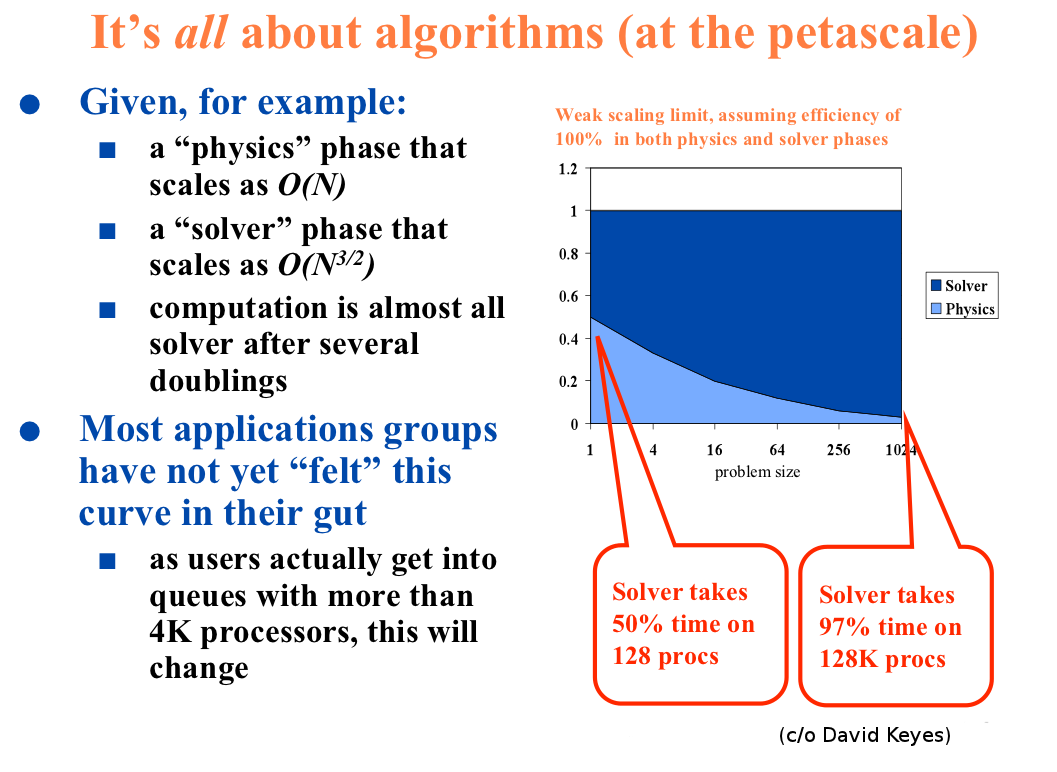
\includegraphics[width=1.1\textwidth]{figures/KeyesAllAboutAlgorithms}
\end{frame}

\section[Hydrostatic]{A robust multigrid solver for the hydrostatic equations}
\begin{frame}[shrink=5]{Hydrostatic equations for ice sheet flow}
  \begin{itemize}
  \item Valid when $w_x \ll u_z$, independent of basal friction {\small (Schoof\&Hindmarsh 2010)}
  \item Eliminate $p$ and $w$ from Stokes by incompressibility:\\
    \quad 3D elliptic system for $\bm u = (u,v)$
    \begin{align*}
      - \nabla\cdot \left[ \eta
        \begin{pmatrix}
          4 u_x + 2 v_y & u_y + v_x & u_z \\
          u_y + v_x & 2 u_x + 4 v_y & v_z
        \end{pmatrix} \right] + \rho g \bar\nabla h & = 0
    \end{align*}
    \begin{align*}
      \eta(\theta,\gamma) &= \frac{B(\theta)}{2} (\gamma_0 + \gamma)^{\frac{1-\mathfrak n}{2\mathfrak n}}, \qquad \mathfrak n \approx 3 \\
      \gamma &= u_x^2 + v_y^2 + u_xv_y + \frac 1 4 (u_y+v_x)^2 + \frac 1 4 u_z^2 + \frac 1 4 v_z^2
    \end{align*}
    and slip boundary $\sigma \cdot \bm n = \beta^2 \bm u$ where
    \begin{align*}
      \beta^2(\gamma_b) &= \beta_0^2 (\epsilon_b^2 + \gamma_b)^{\frac{\mathfrak m-1}{2}}, \qquad 0 < \mathfrak m \le 1 \\
      \gamma_b &= \frac 1 2 (u^2 + v^2)
    \end{align*}
  \item $Q_1$ FEM with Newton-Krylov-Multigrid solver in PETSc: \code{src/snes/examples/tutorials/ex48.c}
  \end{itemize}
\end{frame}

%\frame{
  \vspace{-8em}
  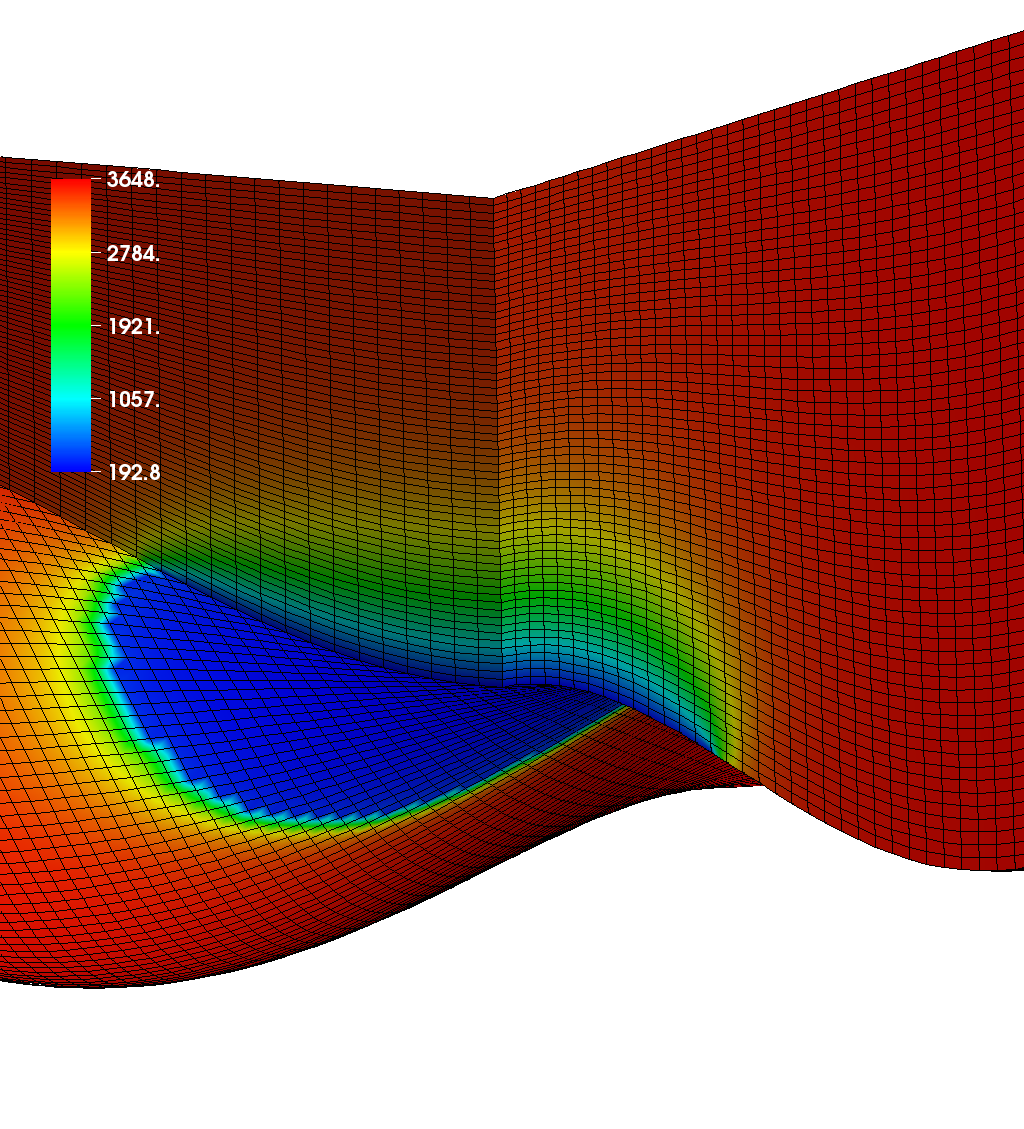
\includegraphics[width=1.2\textwidth]{figures/THI/x-5km-m8p5l5-clip}
}

\begin{frame}
  \includegraphics[width=\textwidth]{figures/THI/x-shear}
\end{frame}
\begin{frame}
  \includegraphics[width=\textwidth]{figures/THI/x-80km-m16p2l6-ew} \\
  Grid-sequenced Newton-Krylov solution of test $X$.  The solid lines denote nonlinear iterations, and the dotted lines with $\times$ denote linear residuals.
\end{frame}
\frame{
  \vspace{-1em}
  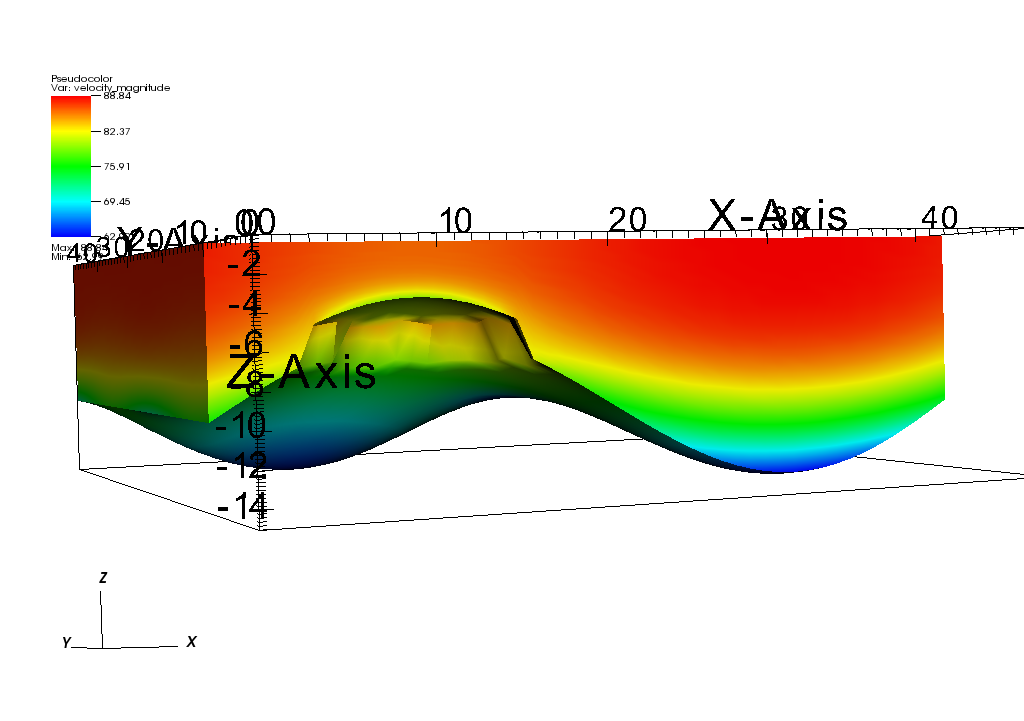
\includegraphics[width=\textwidth]{figures/THI/y-5km-m6p5l4-clip}
  \vspace{-3.5em}
  \begin{itemize}
  \item Bathymetry is essentially discontinuous on any grid
  \item Shallow ice approximation produces oscillatory solutions
  \item Nonlinear and linear solvers have major problems or fail
  \item Grid sequenced Newton-Krylov multigrid works \\
    as well as in the smooth case
  \end{itemize}
}

\begin{frame}
  \begin{figure}
    \includegraphics[width=\textwidth]{figures/THI/y-10km-m10p6l5-ew}
    \centering\caption{Grid sequenced Newton-Krylov convergence for test $Y$.
    The ``cliff'' has \SI{58}{\degree} angle in the red line ($12\times 125$ meter elements), \SI{73}{\degree} for the cyan line ($6\times 62$ meter elements).}\label{fig:testy}
  \end{figure}
\end{frame}
\begin{frame}
  \begin{figure}
    \includegraphics[width=\textwidth]{figures/THI/linear4}
    \centering\caption{Average number of Krylov iterations per nonlinear iteration.  Each nonlinear system was solved to a relative tolerance of $10^{-2}$.}\label{fig:linear}
  \end{figure}
\end{frame}

\begin{frame}
  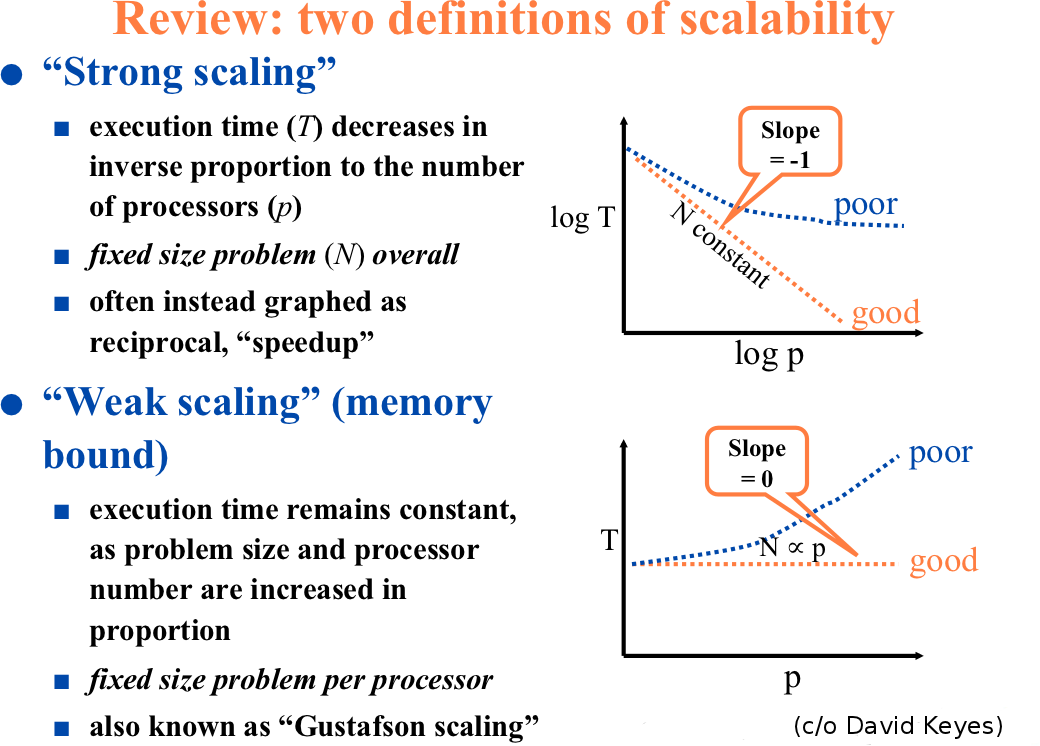
\includegraphics[width=\textwidth]{figures/KeyesStrongWeak}
\end{frame}
\begin{frame}{Strong scaling on Blue Gene/P (Shaheen)}
\begin{figure}
  \includegraphics[width=\textwidth]{figures/THI/shaheen-strong}
  \centering\caption{Strong scaling on Shaheen for different size coarse levels problems and different coarse level solvers.
    The straight lines on the strong scaling plot have slope $-1$ which is optimal.}\label{fig:shaheen-strong}
\end{figure}
\end{frame}

\begin{frame}{Weak scaling on Blue Gene/P (Shaheen)}
  \begin{figure}
  \includegraphics[width=\textwidth]{figures/THI/shaheen-weak}
  \centering\caption{Weak scaling on Shaheen with a breakdown of time spent in different phases of the solution process.
    Times are for the full grid-sequenced problem, not just the finest level solve.}\label{fig:shaheen-weak}
\end{figure}
\end{frame}

\begin{frame}
  \begin{center}
    \alert{\Huge One high-accuracy solve \\

      costs 30 times as much

      \medskip

      as a residual evaluation}
  \end{center}
  \begin{center}
    about 15 to reach truncation error

    \bigskip

    \uncover<2>{\alert{\Large 1000 times faster than existing methods}}
    
    \bigskip

    \uncover<2>{(Brown, Smith, Ahmadia 2011; submitted to JGR)}
  \end{center}
\end{frame}

\section{Other models}
\begin{frame}{Standard shallow approximations}
  \begin{itemize}
  \item Shallow Ice Approximation (SIA):
    \begin{itemize}
    \item Purely local definition of velocity
      \begin{align*}
        u(z) &= - (\rho g)^{\mathfrak n} \int_b^z A(T(z))
        (h-z)^{\mathfrak n} \abs{\bar\nabla h}^{\mathfrak n-1} \bar\nabla h
      \end{align*}
    \item No membrane stresses so only acceptable for \alert<2>{$\lambda \gg 1$}
    \item No solve so costs similar to one residual evaluation per time step
    \end{itemize}
  \item ``Shelfy Stream'' Approximation (SSA)
    \begin{itemize}
    \item Need to solve elliptic problem posed in the map plane (2D):
      \begin{gather*}
        -\bar\nabla\cdot \left[H \bar\eta
          \begin{pmatrix}
            4\bar u_x + 2\bar v_y & \bar v_x + \bar u_y \\
            \bar v_x + \bar u_y   & 2\bar u_x + 4\bar v_y
          \end{pmatrix} \right]
        + \beta^2 \bm{\bar u} + \rho g H \bar\grad h = 0 \\
        \eta(\theta,\gamma) = \frac{B(\theta)}{2} (\gamma_0 + \gamma)^{\frac{1-\mathfrak n}{2\mathfrak n}}, \qquad \mathfrak n \approx 3 \\
        \gamma = \bar u_x^2 + \bar v_y^2 + \bar u_x\bar v_y + \frac 1 4 (\bar u_y+\bar v_x)^2 %{\color{gray} + \frac 1 4 u_z^2 + \frac 1 4 v_z^2}
      \end{gather*}
    \item No vertical shear so only acceptable when \alert<2>{$\lambda \ll 1$}
    \end{itemize}
  \end{itemize}
\end{frame}

\begin{frame}{Vertically-integrated Hybrids}
  \begin{itemize}
  \item Daniel Goldberg 2010, same order of accuracy as hydrostatic
    \begin{itemize}
    \item Vertically average ``membrane'' part of hydrostatic equations
      \begin{gather*}
        -\bar\nabla\cdot \left[\bar\eta
          \begin{pmatrix}
            4\bar u_x + 2\bar v_y & \bar v_x + \bar u_y   \\
            \bar v_x + \bar u_y   & 2\bar u_x + 4\bar v_y
          \end{pmatrix} \right]
        {\color{red} - \left[ \eta \begin{pmatrix} u_z \\ v_z \end{pmatrix} \right]_z}
        + \beta^2 \bm{\bar u} + \rho g H \bar\grad h = 0 \\
        \eta(\theta,\gamma) = \frac{B(\theta)}{2} (\gamma_0 + \gamma)^{\frac{1-\mathfrak n}{2\mathfrak n}}, \qquad \mathfrak n \approx 3 \\
        \gamma = \bar u_x^2 + \bar v_y^2 + \bar u_x\bar v_y + \frac 1 4 (\bar u_y+\bar v_x)^2 {\color{red} + \frac 1 4 u_z^2 + \frac 1 4 v_z^2}
      \end{gather*}
    \item Solve by integrating $z$-dependence and $\eta$, solve linear elliptic problem in map plane for $\bm{\bar u}$, iterate (Picard, $\approx 50$ its)
    \item Evaluating viscosity (or a Newton residual) costs about \\ one hydrostatic residual
    \end{itemize}
  \item Bueler and Brown 2009, used in PISM
    \begin{itemize}
    \item Ad-hoc combination of independent SSA and SIA solutions
    \item Lower formal order of accuracy, but nonlinear solve is strictly 2D
    \end{itemize}
  \end{itemize}
\end{frame}

\begin{frame}{Non-Newtonian Stokes system: velocity $\bm u$, pressure $p$}
\begin{columns}
\begin{column}{0.5\textwidth}
  \alert{\begin{align*}
    -\nabla \cdot(\eta D\uu) + \nabla p - \ff &= 0 \\
    \nabla \cdot \uu &= 0
  \end{align*}}
\end{column}
\begin{column}{0.5\textwidth}
    \begin{align*}
      D\uu &= \tfrac 1 2 \left(\nabla \uu + (\nabla \uu)^T \right) \\
      \gamma(D\uu) &= \tfrac 1 2 D\uu \tcolon D\uu \\
      \eta(\gamma) &= B(\theta,\dotsc)\big(\gamma_0 + \gamma \big)^{\frac{\mathfrak{p}-2}{2}} \\
      \mathfrak{p} &= 1 + \tfrac{1}{\mathfrak{n}} \approx \tfrac 4 3 \\
      T &= \bm 1 - \bm n \otimes \bm n \\
    \end{align*}
\end{column}
\end{columns}
\vspace{-1.5em}
    with boundary conditions
    \begin{align*}
      (\eta D\bm u - p\bm 1)\cdot\bm n =
      \begin{cases}\bm 0 & \text{free surface} \\
        -\rho_w z \bm n & \text{ice-ocean interface}\end{cases} \\
      \bm u = \bm 0\qquad\qquad \text{frozen bed}, \theta < \theta_0 \\
      \left. \begin{aligned}
          \bm u \cdot \bm n &= \bm g_{\text{melt}}(T\uu,\dotsc) \\
          T (\eta D\bm u - p\bm 1)\cdot\bm n &= \bm g_{\text{slip}}(T \bm u,\dotsc) \end{aligned}\right\}
      \text{nonlinear slip}, \theta \ge \theta_0 \\
    \end{align*}
    \vspace{-3em}
    \[ \bm g_{\text{slip}}(T\uu) = \beta_{\mathfrak{m}}(\dotsc) \lvert T\bm u \rvert^{\mathfrak{m}-1} T \bm u \]
    Navier $\mathfrak{m}=1$, \quad Weertman $\mathfrak{m}\approx \frac 1 3$, \quad Coulomb $\mathfrak{m}=0$.
\end{frame}

\begin{frame}{Stokes challenges}
  \begin{block}{Mass conservation is critical}
    \begin{itemize}
    \item Staggered grid finite difference (hard to deal with geometry)
    \item Stabilized methods (conservation artifacts when non-smooth)
    \item Inf-sup stable mixed finite element method
      \begin{itemize}
      \item Use discontinuous pressure to enforce local mass conservation
      \item Inf-sup constant decays like $\sqrt{\epsilon}$ for $Q_k-P_{k-1}^{\text{disc}}$
      \item Sub-optimal order of accuracy for $Q_k-Q_{k-2}^{\text{disc}}$
      \end{itemize}
    \end{itemize}      
  \end{block}
  \begin{block}{Solving saddle-point problems}
    \begin{itemize}
    \item Not uniformly elliptic: solvers are much less robust
    \item Standard preconditioners do not work
    \item Coupled multigrid with Vanka smoothers offer best performance,\\
      \quad not robust for stretched grids or anisotropic viscosity
    \item Block preconditioners require approximate commutators, \\
      \quad fragile for strong anisotropy and non-smooth viscosity
    \end{itemize}
  \end{block}
\end{frame}

\begin{frame}{Outlook}
  \begin{block}{}
    \begin{itemize}
    \item We have textbook multigrid efficiency for hydrostatic equations
    \item All other models are currently slower at high resolution \\ \quad because there are no scalable implementations
    \item Daniel Goldberg's model could be as much as 4 times faster, \\ \quad probably closer to 2 times
    \item Bueler \& Brown's model (or SSA) could be up to 10 times faster
    \item Technical challenges for Stokes
    \item Bathymetry is rough enough that we should solve Stokes
    \item Singularities: reentrant corners, transition from frozen \\ \quad 
      to slip bounadry conditions, grounded margins, grounding lines
    \item Implicit time integration
    \end{itemize}    
  \end{block}
  % \begin{block}{Tools}
  %   \begin{itemize}
  %   \item PETSc\ \url{http://mcs.anl.gov/petsc}
  %     \begin{itemize}\item ML, Hypre, MUMPS
  %     \end{itemize}
  %   \item ITAPS \url{http://itaps.org}
  %     \begin{itemize}\item MOAB, CGM, Lasso
  %     \end{itemize}
  %   \end{itemize}
  % \end{block}
\end{frame}

\begin{frame}
  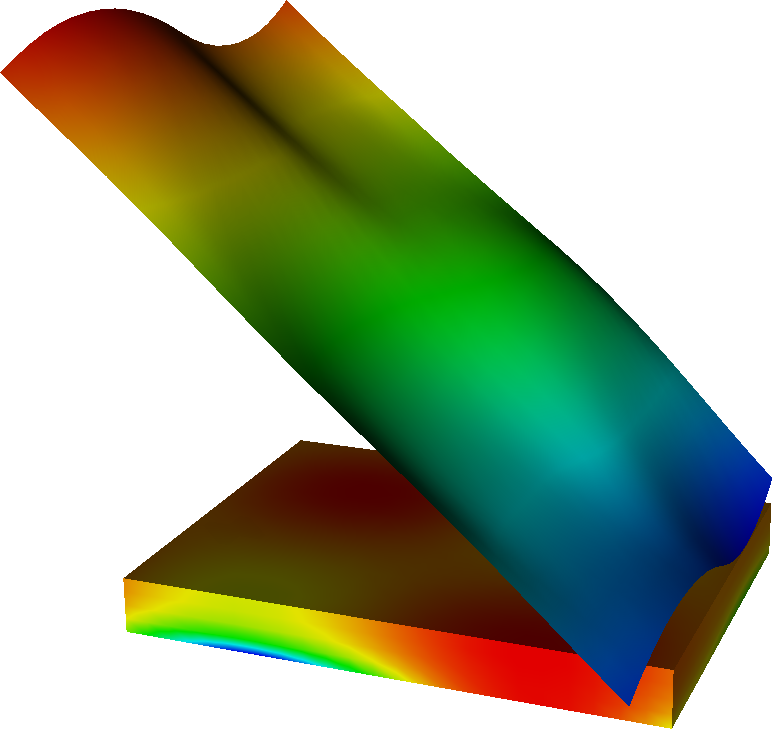
\includegraphics[width=0.5\textwidth]{figures/THI/c-steady-crop}
  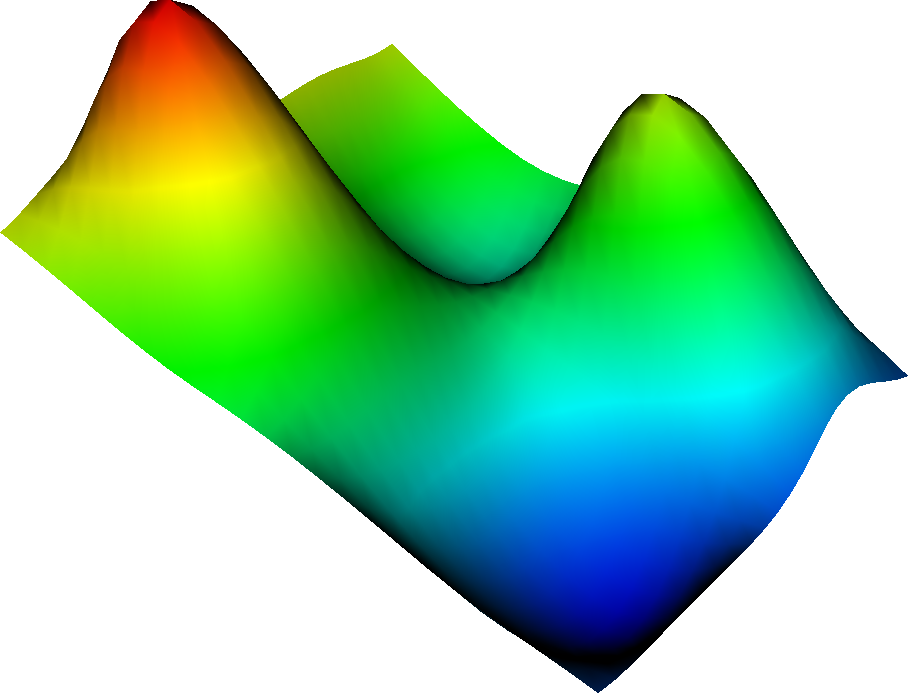
\includegraphics[width=0.5\textwidth]{figures/THI/erosion300k}
\end{frame}
\end{document}
